% #############################################################################
% This is Chapter 1
% !TEX root = main.tex
% #############################################################################
% Change the Name of the Chapter i the following line
\fancychapter{Introduction}
\clearpage
% The following line allows to ref this chapter
\label{chap:chap001}
\noindent

This section presents the work motivation, goals, and contributions of this dissertation thesis in the context of my doctoral program.
The work described in this document started in September 2015, before and during my Master Thesis, founded by a research grant from \ac{FCT}.
The funding was provided under the \ac{RD} Units Strategic Plan - 2013/2015 - \ac{OE}, with the UID/EEA/50009/2013 reference.
The official starting date of my \ac{PhD} program in \ac{CSE} at \ac{IST} of \ac{UL} is September 2018 and since January 2020 that my work has been funded by \ac{FCT} with the grant PD/BD/150629/2020 reference.

\section{Motivation}
\label{sec:chap001001}

Breast cancer is the second leading cause of death from cancer in women~\cite{https://doi.org/10.3322/caac.21754}.
However, early detection and treatment can considerably improve results~\cite{doi:10.1002/cncr.32859}.
Consequently, large-scale screening programs are implemented worldwide.
Most medical and governmental organizations recommend screening for all women between 40 and 50 of age~\cite{https://doi.org/10.3322/caac.21754}.
The annual incidence of over 400,000 new female cases in Europe~\cite{Dafni2019} underscores the pressing requirement.
Therefore, efficient screening and diagnostic methods are essential in addressing this challenge.

Despite the extensive adoption of screening exams, interpreting these images remains challenging.
The accuracy achieved by clinical experts in cancer detection varies widely (Figure~\ref{fig:fig114}), and the performance of even the best clinicians leaves room for improvement~\cite{10.1001/jamainternmed.2015.5231}.
For instance, the \acp{FP}\footnotemark[1] can lead to the anxiety of the patient~\cite{10.1001/jamainternmed.2014.981}, avoidable follow-ups, and unnecessary procedures of invasive diagnostics.
On the other hand, the \acp{FN}\footnotemark[2] are even more severe, since the exam misdiagnoses a patient who has the disease~\cite{doi:10.1056/NEJMe1912943}.
During the screening phase, the missing cancers may not be identified until they are more advanced and less agreeable to treatment~\cite{Houssami2017}.

%%%%%%%%%%%%%%%%%%%%%%%%%%%%%%%%%%%%%%%%%%%%%%%%%%%
\footnotetext[1]{False-Positive: when the screening result looks abnormal even though no cancer is actually present. Abnormal screening results often require extra testing to determine if the change is cancer. The FP results are more common in younger women, who have dense breasts, have had breast biopsies, have breast cancer in the family, or are taking estrogen.}
%%%%%%%%%%%%%%%%%%%%%%%%%%%%%%%%%%%%%%%%%%%%%%%%%%%

%%%%%%%%%%%%%%%%%%%%%%%%%%%%%%%%%%%%%%%%%%%%%%%%%%%
\footnotetext[2]{False-Negative: when the screening result looks normal even though breast cancer is present. Women with dense breasts are likelier to get FN results. The FN cases can give women a false sense of security, thinking that they don’t have breast cancer, when in fact, they do.}
%%%%%%%%%%%%%%%%%%%%%%%%%%%%%%%%%%%%%%%%%%%%%%%%%%%

The integration of \ac{AI} in medical imaging workflows presents a unique opportunity to address this challenge~\cite{McKinney2020}, leveraging technologies such as {\it radiomics}, \ac{CADe}, \ac{CADx}, \acp{CDSSe} inside the \ac{RRR}.
Extensive research has demonstrated the potential of \ac{AI} to achieve or even surpass human performance in various clinical tasks, offering promising avenues for enhancing healthcare delivery\cite{Topol2019}.
Given the global shortage of medical professionals, which threatens the adequacy and accessibility of clinical services, the scalability of \ac{AI} solutions holds the potential to elevate the standard of care and bridge the gap in healthcare provision~\cite{McKinney2020, Topol2019}.

%%%%%%%%%%%%%%%%%%%%%%%%%%%%%%%%%%%%%%%%%%%%%%%%%%%
\begin{figure}[ht]
\centering
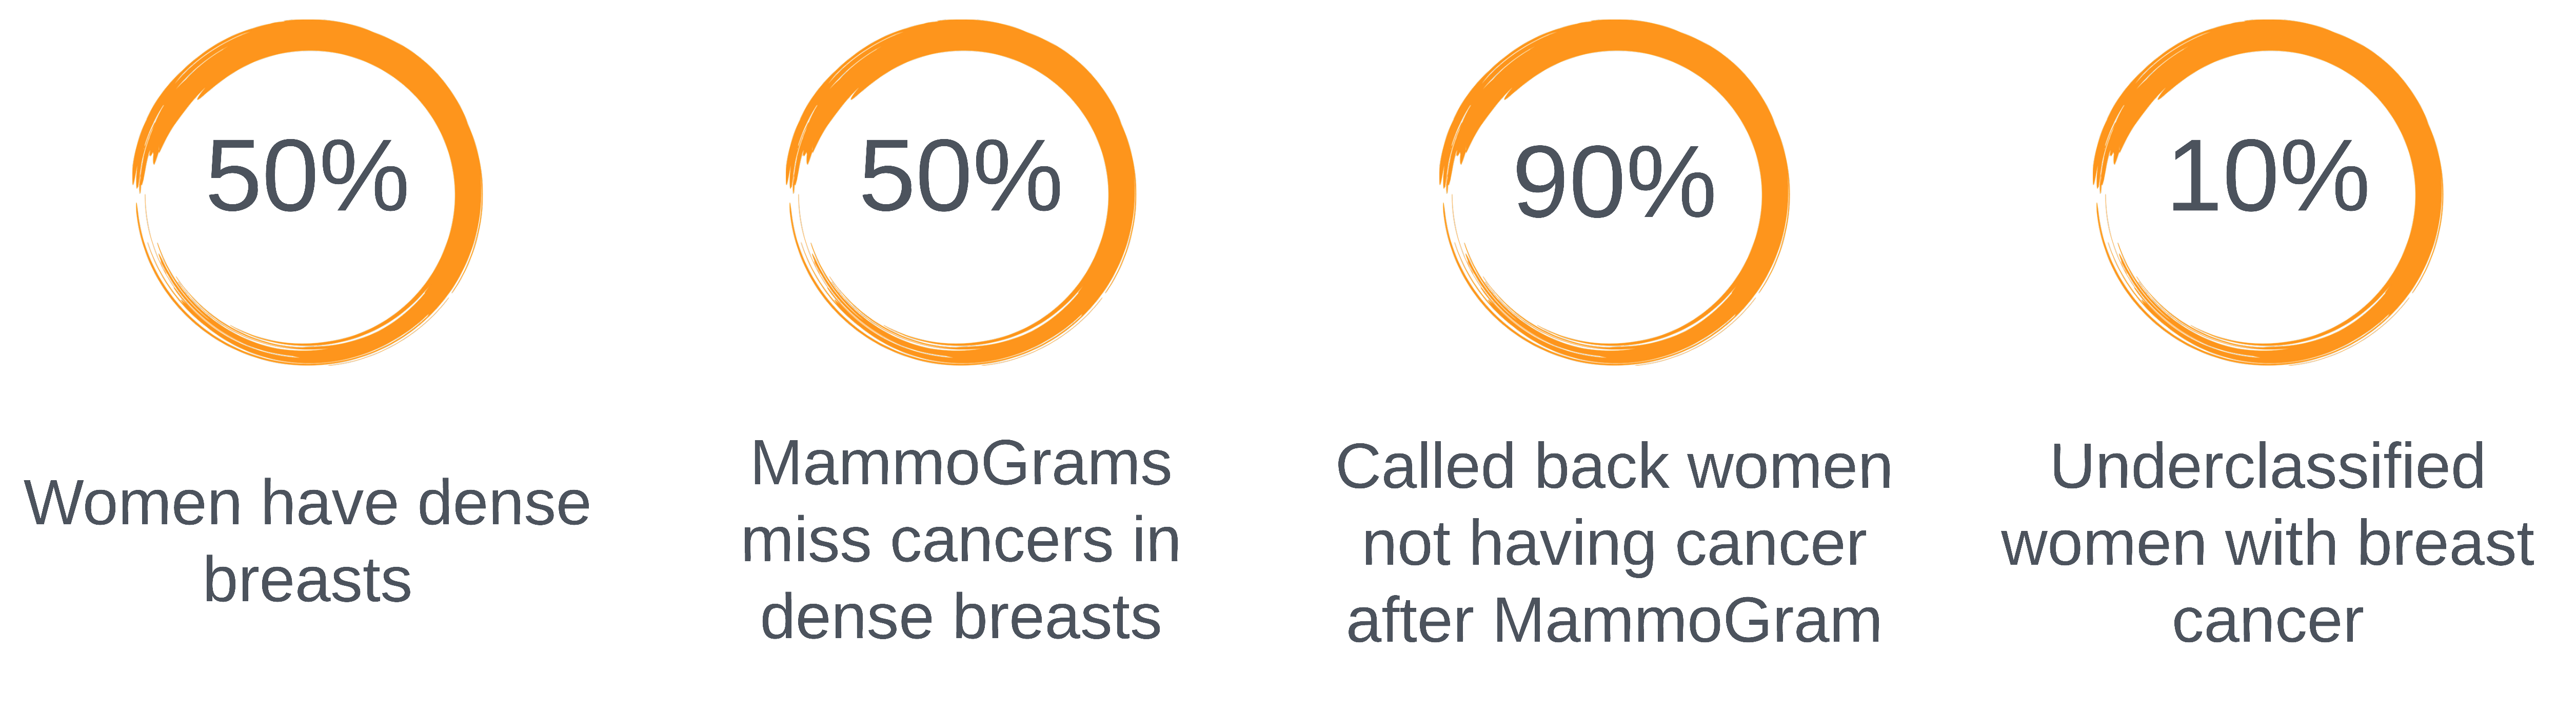
\includegraphics[width=\textwidth]{images/fig114}
\caption{Proportions of breast cancer patients with missing cases and distribution among screened patients. Approximately 1 in 2 women have dense breasts, while dense breasts have 50\% chance of missing a cancer. FPs in breast screening are quite common, with around 90\% of women who are called back for further exams after a MG not having cancer. Additionally, about 10\% of breast cancers are underclassified or misclassified as negative (FN) when they are actually positive, which can have serious consequences for patients. Source: National Cancer Institute (\href{https://www.cancer.gov/types/breast/mammograms-fact-sheet}{cancer.gov}). Retrieved on July 3, 2023.}
\label{fig:fig114}
\end{figure}
%%%%%%%%%%%%%%%%%%%%%%%%%%%%%%%%%%%%%%%%%%%%%%%%%%%

In the medical imaging domains, \ac{AI} has the potential to improve visual diagnostic accuracy~\cite{Tschandl2020}.
\ac{AI}-based triage and decision support could assist readers, such as radiologists, in managing clinical workflows and improving their performance~\cite{McKinney2020}.
Most recent works have been predicted on comparisons of the diagnostic accuracy of \ac{AI} systems with clinicians~\cite{He2019, 10.1145/3313831.3376290}.
Furthermore, recent studies, in breast cancer, demonstrate that \ac{AI} for diagnosis is equivalent or even superior to human experts in medical imaging under experimental conditions~\cite{Ribli2018, McKinney2020}.
This competitive view of \ac{AI} is evolving based on studies suggesting that a more promising approach is an \ac{HAII}~\cite{10.1145/3313831.3376807, 10.1145/3313831.3376301}, with techniques that improve the interaction between humans and machines.

The role of \ac{HAII} in healthcare delivery and its impact on the quality of care, as well as the appropriate settings in which it can be applied, are critical areas that require evaluation~\cite{Tschandl2020}.
Furthermore, in the context of \ac{DL} models, the `black box' nature of these models raises concerns regarding the transparency and interpretability of their decisions~\cite{9473208}.
To address this challenge, it is essential to understand the underlying representations and explanations generated by these models, as this knowledge is crucial for instilling trust and fostering acceptance among healthcare professionals and patients~\cite{10.1145/3544548.3581075, EVANS2022281}.
Although researchers have made attempts to study the effects of \ac{HAII} across different clinical workflows and levels of medical expertise~\cite{doi:10.1148/radiol.2019182627}, there is still a lack of understanding regarding personalized and customized \ac{AI} recommendations.
The final objective of this thesis is to address this gap by adapting \ac{AI} recommendations to various representations and explanations generated by \ac{DL}-based classifiers, an area that has not been extensively explored.
This involves using anthropomorphic intelligent agents with human-like qualities, behaviors, and characteristics.
In our dissertation, these intelligent agents act as second readers, offering diagnostic support and emulating clinicians' reasoning.
Therefore, this research gap presents an open opportunity for investigation, serving as the motivation behind the proposed research in this thesis.

\section{Research View}
\label{sec:chap001002}

Our work aims to enhance clinicians' understanding and acceptance of \ac{AI} systems by leveraging recent advancements in \ac{DL} methods and studying their applicability across different levels of medical expertise and clinical workflows.
In Section~\ref{sec:chap001002001}, we provide a detailed overview of the specific areas that our dissertation will encompass.
Following that, in Section~\ref{sec:chap001002002}, we outline the main objectives for each chapter of the dissertation.
Together, these sections intertwine to establish a robust foundation as the fundamental bedrock for our comprehensive investigation, providing essential support and guidance to our dissertation thesis.

\subsection{Research Scope}
\label{sec:chap001002001}

This dissertation delves into the design, development, and assessment of novel \ac{AI}-based visual representations, particularly in medical imaging diagnosis (Section~\ref{sec:chap002001}).
The work builds on recent advancements in the accuracy of \ac{DL} methods~\cite{9098470}, studying their utility across various levels of medical expertise and numerous clinical workflows (Section~\ref{sec:chap002002}).
Despite the potential to assist clinicians, challenges persist, namely the scarcity of available, curated medical data~\cite{10.1145/3313831.3376290}, and the opacity of \ac{AI} decision-making processes~\cite{Yue_2020_CVPR}.
To counter these, the thesis proposes a dual approach:
(1) developing a {\it framework} to support the visualization of clinical findings provided by \ac{DL} methods for severity classification of a patient (Section~\ref{sec:chap002003}); and
(2) enhancing clinicians' comprehension about \ac{AI} algorithmic results through granular explanations of the medical data, for instance, informing the lesion typification (Section~\ref{sec:chap002004}) that will clarify the severity of that patient.
While considering this process within the workflow context (Section~\ref{sec:chap002005}), the dissertation also recognizes the importance of rendering multi-modal images\footnotemark[3] and other \ac{AI} techniques (Section~\ref{sec:chap002006}).
Ultimately, the thesis advocates for a user-centric intelligent agent that mimics human reasoning, despite certain complexities (Section~\ref{sec:chap002007} and Section~\ref{sec:chap002008}), to facilitate a more straightforward interpretation of the \ac{DL} outcomes for clinicians.

%%%%%%%%%%%%%%%%%%%%%%%%%%%%%%%%%%%%%%%%%%%%%%%%%%%
\footnotetext[3]{Multimodality: in this thesis, a diagnostic technique for the patient treatment: (1) \ac{MG}, both \ac{CC} and \ac{MLO} views; (2) \ac{US}; (3) \ac{MRI}; and (4) text. The considered text modalities are, for instance, report information, personal history, family history, and age, among others.}
%%%%%%%%%%%%%%%%%%%%%%%%%%%%%%%%%%%%%%%%%%%%%%%%%%%

The primary objective of this dissertation is to make a meaningful contribution to the intersection of \ac{HCI} and \ac{AI} in medical systems by tackling existing challenges (Section~\ref{sec:chap003001}) and harnessing the possibilities offered by anthropomorphic intelligent agents in the context of medical imaging diagnosis.
Through the application of \ac{UCD} principles and the utilization of methodologies such as user research, usability testing, and cognitive task analysis, the thesis strives to improve the user-friendliness, efficacy, and transparency of \ac{AI} systems in medicine.
The overarching objective is to develop \ac{AI} solutions that effectively address the requirements of healthcare professionals and enhance the diagnostic process in medical imaging.

\subsection{Research Objectives}
\label{sec:chap001002002}

This dissertation aims to thoroughly investigate the adoption, acceptance, and impact of intelligent agents within the field of \ac{HCI} and specifically in medical imaging.
The primary objective is to explore integrating intelligent agents into the medical imaging workflow and understand their influence on clinicians' acceptance and utilization of \ac{AI} systems.
Additionally, the dissertation examines the overall consequences of adopting intelligent agents in the medical imaging domain, providing valuable insights into the potential benefits and challenges associated with their implementation.

\vspace{2.00mm}

\noindent
The research objectives for each chapter are outlined below:

\vspace{1.00mm}

\begin{enumerate}
\item Adoption and Acceptance of Intelligent Agents in the Medical Imaging Workflow (Chapter~\ref{chap:chap004});
\begin{enumerate}[label*=\arabic*.]
\item Investigate how intelligent agents impact technology adoption in medical imaging and understand their influence on clinicians' acceptance of \ac{AI} systems.
\item Explore the determinants of trust and acceptance in clinicians' technology usage, identifying the factors influencing their adoption of \ac{AI} systems in the medical imaging workflow.
\item Improve the explanatory power of a questionnaire based on the \ac{UTAUT} constructs for assessing clinicians' intentions to use \ac{AI} systems in the context of medical imaging.
\end{enumerate}
\item Design Interventions and \ac{AI} Assistance in Radiology (Chapter~\ref{chap:chap005});
\begin{enumerate}[label*=\arabic*.]
\item Enhance clinicians' understanding and trust of \ac{AI} recommendations and explanations in clinical decision-making, incorporating design techniques through a human-centered approach.
\item Incorporate design interventions to effectively introduce \ac{AI} systems and enhance clinicians' satisfaction, acceptance, and overall experience with intelligent agents in radiology.
\item Assess the effects of \ac{AI} assistance on the medical workflow, encompassing improvements in diagnostic accuracy, time performance, and consistency in patient classification.
\end{enumerate}
\item Personalized Communication of \ac{AI}-Assisted Systems (Chapter~\ref{chap:chap006});
\begin{enumerate}[label*=\arabic*.]
\item Understand clinicians' perceptions of assertiveness-based agents, considering their expertise and familiarity with \ac{AI}-assisted systems.
\item Analyze the impact of personalized and assertiveness-based communication on medical assessments, aiming to understand its influence on clinicians' decision-making, patient diagnosis efficiency, and overall workflow performance.
\item Delve into how assertiveness-based agents influence efficiency, accuracy, perception, and usability among clinicians, aiming to assess their effectiveness and perceived trustworthiness.
\end{enumerate}
\end{enumerate}

\section{Thesis Statement}
\label{sec:chap001003}

\noindent
This dissertation aims to defend the following thesis statement:

\begin{quote}
{\it
Augmented medicine empowers clinicians' decision-making by leveraging sophisticated computation and inference to generate insights, as well as autonomous recommendations, where \ac{AI} promises to revolutionize the healthcare sector.
\ac{AI} has the potential to be used in the detection and characterization of several medical diseases.
Through a human-centered design, the outcome of this dissertation aims to significantly improve the efficiency of the diagnostic process for cancer patients by reducing the waiting time from weeks to days, which is critical given the time-sensitivity of cancer treatments.
Additionally, it can reduce the workload of radiologists by decreasing the number of exams to be analyzed by half.
Broader adaptation and customization of the \ac{AI} outcomes may augment individual clinicians to higher cancer detection rates, as well as a reduction of cost and risk for the patient.
As appealing concepts, personalizing and customizing the \ac{AI} outcomes for each clinician will promote a better understanding of \ac{AI} predictions and explain why \ac{AI} achieved some results.
}
\end{quote}

\noindent
To defend this statement, the remainder of this dissertation addresses the following research questions:

\begin{enumerate}
\item How can intelligent agents be successfully designed, motivating clinicians to accept and adopt \ac{AI}-based systems in radiology?
\begin{enumerate}
\item How do the factors influencing clinicians' acceptance and adoption of intelligent agents in radiology manifest in practice?
\item How do clinicians perceive the potential benefits and drawbacks of adopting intelligent agents in radiology?
\item How can we design and implement effective strategies for encouraging clinicians' acceptance and adoption of intelligent agents in radiology?
\end{enumerate}
\item How can \ac{AI} assistance be designed and implemented to effectively improve the clinical workflow and diagnostic interpretability for clinicians in radiology?
\begin{enumerate}
\item How can we incorporate design interventions to effectively introduce \ac{AI} systems and enhance clinicians' satisfaction, acceptance, and overall experience with intelligent agents in radiology?
\item How should explainability be designed for setting appropriate expectations of clinicians and to improve diagnostic interpretability over an AI recommendation?
\item How does AI assistance impact clinicians' workflow for avoiding different types of diagnostics?
\end{enumerate}
\item How can personalization and customization be optimized to enhance medical assessments and improve clinicians' perceptions of the intelligent agents?
\begin{enumerate}
\item How does a personalized and customized intelligent agent affect medical assessments?
\item How do clinicians perceive a personalized and customized intelligent agent?
\end{enumerate}
\end{enumerate}

\section{Thesis Overview}
\label{sec:chap001004}

Here, we provide an overview of the research conducted in this dissertation.
The main body of the dissertation (Section~\ref{sec:chap001004001}) consists of chapters dedicated to substantiating our thesis statement.
Additional descriptions (Section~\ref{sec:chap001004002}) provide more detailed information on these chapters.
We also present complementary information (Section~\ref{sec:chap001004003}), including questionnaires, \ac{UTA} guides, as well as technical details of the framework and its current market stage.
These supplementary materials are included alongside each chapter to tackle our research problems (Section~\ref{sec:chap001004004}).

\subsection{Thesis Core}
\label{sec:chap001004001}

In this section, we offer the core skeleton of the thesis.
We explore the relevant background context and pertinent literature that form the foundation for our work (Chapter~\ref{chap:chap002} and Chapter~\ref{chap:chap003}).
Subsequently, we present chapters that contribute to our objective of enhancing the adoption of intelligent agents (Chapter~\ref{chap:chap004}) through a human-centered design approach (Chapter~\ref{chap:chap005}) and personalizing clinicians' decision-making (Chapter~\ref{chap:chap006}).
Finally, we discuss (Chapter~\ref{chap:chap007}) and conclude (Chapter~\ref{chap:chap008}) our main findings, revealing general design recommendations and principles.

\vspace{2.00mm}

\noindent
{\bf Chapter~\ref{chap:chap002}}:
We provide a concise overview of the medical imaging background and the current clinical workflow.
We aim to highlight the opportunities for research and development of intelligent agents in this medical workflow.
Additionally, Appendix~\ref{chap:app001} extends a more comprehensive elaboration of the chapter.

\vspace{2.00mm}

\noindent
{\bf Chapter~\ref{chap:chap003}}:
This chapter of our dissertation offers a thorough literature review and explores recent developments in the field of \ac{HCI} about \ac{AI}-assisted medical decision-making.
In conjunction with Chapter~\ref{chap:chap002} and Appendix~\ref{chap:app001}, this chapter accomplishes our literature review goal.
Together, these components provide valuable insights into the medical background and critically analyze the relevant \ac{HCI} literature.

\vspace{2.00mm}

\noindent
{\bf Chapter~\ref{chap:chap004}}:
The chapter explores factors influencing clinicians' adoption of \ac{AI} in the medical workflow.
In conjunction, Appendix~\ref{chap:app002} expands a complete analysis to complement this chapter.
These components collectively address the acceptance and adoption challenges in medical imaging.

\vspace{2.00mm}

\noindent
{\bf Chapter~\ref{chap:chap005}}:
Explore radiologists' requirements in utilizing \ac{AI}-powered image diagnostics.
Appendix~\ref{chap:app003} offers additional insights to complement this chapter.
It is also essential to address Appendix~\ref{chap:app004}, which discusses the integration of our \ac{DL} models and their architectural implications for designing the final solution.
Jointly, these three components address the challenges related to our human-centered approach.

\vspace{2.00mm}

\noindent
{\bf Chapter~\ref{chap:chap006}}: This chapter explores how \ac{AI} systems should communicate to effectively address the specific needs and characteristics of different user groups.
In addition to this chapter, Appendix~\ref{chap:app005} provides supplementary insights.
Concurrently, these two components tackle the challenges associated with the personalization and customization of intelligent agents in clinical workflows.

\noindent
{\bf Chapter~\ref{chap:chap007}}:
Presents contributions and design recommendations under this thesis.
The findings emphasize the significance of compliant agents providing tailored explanations for future enhancements.
These insights contribute significantly to research in \ac{HCI} and \ac{AI} communication for healthcare.

\vspace{2.00mm}

\noindent
{\bf Chapter~\ref{chap:chap008}}:
Deliver the concluding findings of the dissertation, highlighting design principles.
Combined with Chapter~\ref{chap:chap007}, these chapters pave the way for \ac{AI} integration in healthcare.
Together, they address the final remarks and contributions of this dissertation.


\subsection{Additional Descriptions}
\label{sec:chap001004002}

We have described the core chapters of this dissertation, summarizing our main contributions for simplicity to the reader.
However, more extensive details are presented in the following appendices.

\vspace{2.00mm}

\noindent
{\bf Appendix~\ref{chap:app001}}:
This appendix provides detailed information expanding on the topics in Chapter~\ref{chap:chap002}.
The appendix will provide further information on the clinical processes and medical specifications.

\vspace{2.00mm}

\noindent
{\bf Appendix~\ref{chap:app002}}:
Offers an expanded analysis, building upon the initial description in Chapter~\ref{chap:chap004}.
More results of acceptance and adoption are provided here, such as detailing the moderating effects.

\vspace{2.00mm}

\noindent
{\bf Appendix~\ref{chap:app003}}:
Provides further implications made during Chapter~\ref{chap:chap005} regarding diagnostic performance and accuracy, between others.
The appendix is offering a much more in-depth analysis of this chapter.

\vspace{2.00mm}

\noindent
{\bf Appendix~\ref{chap:app004}}:
Together with Appendix~\ref{chap:app003}, this appendix provides valuable insights into the design process.
It explores the integration of our \ac{DL} models, vital to Chapter~\ref{chap:chap005}.

\vspace{2.00mm}

\noindent
{\bf Appendix~\ref{chap:app005}}:
This appendix offers additional descriptions pertaining to Chapter~\ref{chap:chap006}.
We are offering here additional results and discussion, such as clinicians' performance, preferences, and other insights.

\subsection{Complementary Information}
\label{sec:chap001004003}

In addition, we supplement the thesis with complementary information.
This information will give further details concerning the used questionnaires, \ac{UTA} guides, and {\it framework} details, described next.

\vspace{2.00mm}

\noindent
{\bf Appendix~\ref{chap:app006}}:
The employed questionnaires, {\it e.g.}, demographic data, \acs{SUS}, etc., are provided.
These questionnaires constitute a part of the outcomes derived from Chapter~\ref{chap:chap004}, Chapter~\ref{chap:chap005}, and Chapter~\ref{chap:chap006}.

\vspace{2.00mm}

\noindent
{\bf Appendix~\ref{chap:app007}}:
\ac{UTA} refers to a document that guides the user testing process.
The first document is connected to our 8\textsuperscript{th} \ac{UTA} for Chapter~\ref{chap:chap004}, the second to our 7\textsuperscript{th} \ac{UTA} for Chapter~\ref{chap:chap005}, and the third to our 11\textsuperscript{th} \ac{UTA} for Chapter~\ref{chap:chap006}.
The number progression follows the order of the chapters, not chronological.


\vspace{2.00mm}

\noindent
{\bf Appendix~\ref{chap:app008}}:
This complementary information attaches the technical report that sustains the invention of our basic {\it BreastScreening} framework~\cite{10.1145/3399715.3399744, WO2022071818A1}.
The document provides functionality details and market perspectives for introducing \ac{AI} systems in the healthcare sector.

\subsection{Problems \& Contributions}
\label{sec:chap001004004}

\noindent
The approach towards these goals was divided into five parts (Figure~\ref{fig:fig115}) by showing the thesis problems and respective associated contributions:

\vspace{1.00mm}

%%%%%%%%%%%%%%%%%%%%%%%%%%%%%%%%%%%%%%%%%%%%%%%%%%%
\begin{figure}[ht]
\centering
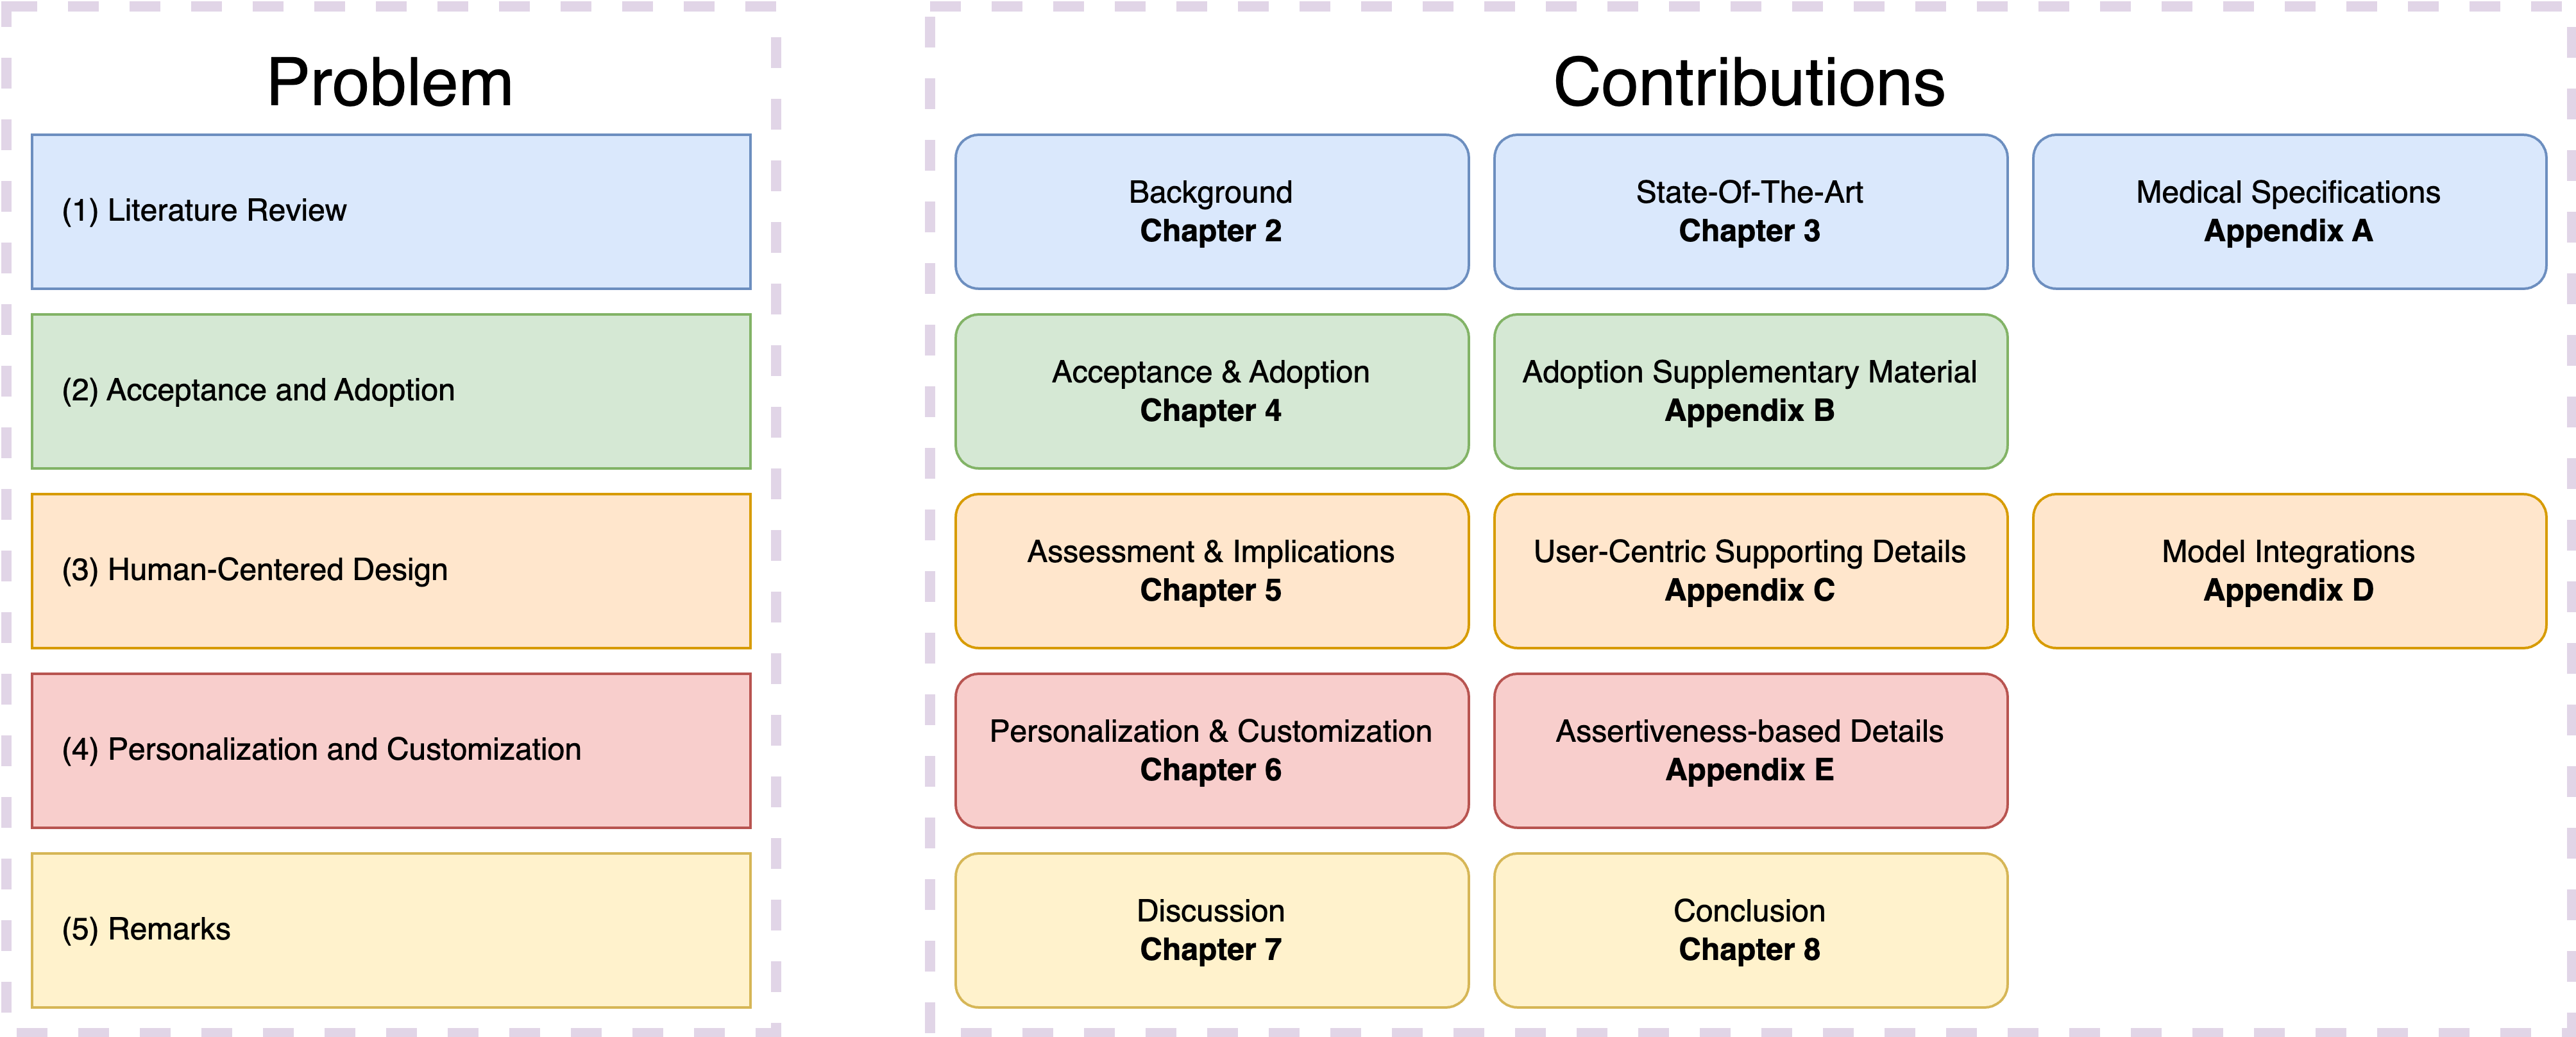
\includegraphics[width=\textwidth]{images/fig115}
\caption{[DOI: \protect\href{https://www.doi.org/10.13140/RG.2.2.14314.95685/2}{10.13140/RG.2.2.14314.95685/2}] Thesis problem and contribution relationships. In this dissertation, five scientific problems were addressed: (1) mitigating the bias between the clinical background of the medical imaging workflow and the related work of intelligent agents among the research communities; (2) understanding the factors influencing AI acceptance and adoption of intelligent agents in medical imaging diagnosis; (3) addressing clinicians' needs and preferences through design interventions that prioritize a human-centered approach to integrate DL models into real-world clinical workflows; (4) supporting evidence for effectively personalize and customize the explanations of intelligent agents based on the behavioral characteristics of clinicians with varying levels of medical expertise; and (5) discussing conclusive recommendations and principles raised from our findings.}
\label{fig:fig115}
\end{figure}
%%%%%%%%%%%%%%%%%%%%%%%%%%%%%%%%%%%%%%%%%%%%%%%%%%%

Several contributions are solving each problem challenge addressed in this thesis (Figure~\ref{fig:fig115}).
Although this dissertation focuses on the main goals and contributions of the thesis, a critical objective is to provide information concerning the medical imaging background and review of the literature for \ac{HCI} related work.
For problem one (Chapter~\ref{chap:chap002}, Chapter~\ref{chap:chap003} and Appendix~\ref{chap:app001}), we aim to improve the understating of clinicians, researchers, engineers, and policymakers in developing robust and effective user-centric interventions across the breast cancer domain.
Moreover, problem two (Chapter~\ref{chap:chap004} and Appendix~\ref{chap:app002}) seeks light on the adoption and acceptance of intelligent agents in the context of the medical imaging workflow.
In problem three (Chapter~\ref{chap:chap005}, Appendix~\ref{chap:app003}, and Appendix~\ref{chap:app004}), we prioritize a human-centered approach to address clinicians' needs and preferences on the integration of \ac{DL} models into real-world clinical workflows through design interventions.
From here, it highlights the clinicians' requirements for functionality improvements and effective communication of the intelligent agents (Chapter~\ref{chap:chap006} and Appendix~\ref{chap:app005}), considering the need for personalizing and customizing \ac{AI} recommendations of problem four.
Ultimately, we discuss and conclude our final remarks on problem five (Chapter~\ref{chap:chap007} and Chapter~\ref{chap:chap008}), while providing design recommendations and principles from our findings.

\section{Research Contributions}
\label{sec:chap001005}

The main contributions achieved so far are the following:

\begin{enumerate}
\item {\bf Factors affecting the acceptance and adoption} of intelligent agents in medical imaging;
\begin{enumerate}[label*=\arabic*.]
\item Investigated {\bf factors affecting the adoption of intelligent agents in medical imaging}, verifying security, risk, and trust as essential antecedents of user acceptance;
\item Identified {\bf moderating relationships} between antecedent factors and behavioral acceptance based on gender, age, and education, between others, exploring how medical experience, training levels, and expertise areas can also moderate these relationships;
\end{enumerate}
\item {\bf Design and evaluation of intelligent agents} in real-world clinical settings;
\begin{enumerate}[label*=\arabic*.]
\item Conducted a study with 45 physicians, evaluating a {\bf BreastScreening prototype} with and without \ac{AI}, and compared the accuracy of the \ac{AI} condition using \ac{FP} and \ac{FN} metrics;
\item Provided {\bf design recommendations} for visualization to support {\it radiomics} in breast cancer;
\item Demonstrated the {\bf impact of multi-modal imaging and \ac{AI}-assisted strategy} in diagnosing and severity classification of lesions;
\item Examined the impact of our {\bf proposed design techniques} on clinicians' expectations and satisfaction when interacting with an intelligent agent;
\end{enumerate}
\item Enhancing clinical workflows and trust through {\bf assertiveness-based agents};
\begin{enumerate}[label*=\arabic*.]
\item Customized \ac{AI}-assisted medical reasoning with {\bf assertiveness-based communication}, enhancing clinical workflows;
\item Probes into the applicability of granular clinical explanations and user confidence in {\bf personalized \ac{AI} recommendations} without undermining diagnostic accuracy;
\item Explored the impact of explaining \ac{AI} outputs on medical efficiency, considering the {\bf communication tone} of clinical arguments;
\item Provided {\bf design considerations for adapting communication} in \ac{AI} reasoning based on medical expertise levels, facilitating the implementation of personalized intelligent agents;
\end{enumerate}
\item We {\bf published novel datasets} containing clinical information, user data, and results.
\end{enumerate}

\section{List of Publications \& Communications}
\label{sec:chap001006}

The work developed in this thesis was published in conferences and journal papers.
The following sections will list the set of publications published until now.

\subsection{Conference Papers}
\label{sec:chap00100601}

\begin{enumerate}
\item {\bf Francisco Maria Calisto}, Jo\~{a}o Fernandes, Margarida Morais, Carlos Santiago, Jo\~{a}o M. Abrantes, Nuno J. Nunes, and Jacinto C. Nascimento. 2023. Assertiveness-based Agent Communication for a Personalized Medicine on Medical Imaging Diagnosis. Proceedings of the 2023 CHI Conference on Human Factors in Computing Systems (CHI '23), April 23--28, 2023, Hamburg, Germany. Association for Computing Machinery, New York, NY, USA, Article 13, 1–20. DOI: \href{https://doi.org/10.1145/3544548.3580682}{doi.org/10.1145/3544548.3580682}
\item Pedro Diogo, Margarida Morais, {\bf Francisco Maria Calisto}, Carlos Santiago, Clara Aleluia and Jacinto C. Nascimento. 2023. Weakly-Supervised Diagnosis and Detection of Breast Cancer using Deep Multiple Instance Learning. 2023 IEEE 20th International Symposium on Biomedical Imaging (ISBI '23), April 18--21, 2023, Cartagena de Indias, Colombia. Institute of Electrical and Electronics Engineers (IEEE), Piscataway, NJ, US, Article {\bf N}, 1–20.
\item Margarida Morais, {\bf Francisco Maria Calisto}, Carlos Santiago, Clara Aleluia and Jacinto C. Nascimento. 2023. Classification of Breast Cancer in MRI with Multimodal Fusion. 2023 IEEE 20th International Symposium on Biomedical Imaging (ISBI '23), April 18--21, 2023, Cartagena de Indias, Colombia. Institute of Electrical and Electronics Engineers (IEEE), Piscataway, NJ, US, Article {\bf N}, 1–20.
\item Jo\~{a}o Maria Abrantes, Maria Jo\~{a}o Bento e Silva, Jos\'{e} Pedro Meneses, Catarina Oliveira, {\bf Francisco Maria Calisto}, Ross Warren Filice. 2023. External Validation of a Deep Learning Model for Breast Density Classification. 2023 European Congress of Radiology (ECR '23), March 1--5, 2023, Viena, Austria. European Society of Radiology, Vienna, Austria. Poster ECR 2023 / C-16014, 1–2. DOI: \href{https://dx.doi.org/10.26044/ecr2023/C-16014}{dx.doi.org/10.26044/ecr2023/C-16014}
\item {\bf Francisco Maria Calisto}, Nuno J. Nunes, and Jacinto C. Nascimento. 2020. BreastScreening: On the Use of Multi-Modality in Medical Imaging Diagnosis. In Proceedings of the International Conference on Advanced Visual Interfaces (AVI '20), September 28 -- October 2, 2020, Ischia Island, Italy. Association for Computing Machinery, New York, NY, USA, Article 49, 1–5. DOI: \href{https://doi.org/10.1145/3399715.3399744}{doi.org/10.1145/3399715.3399744}
\item {\bf Francisco Maria Calisto}, Alfredo Ferreira, Jacinto C. Nascimento, and Daniel Gon\c{c}alves. 2017. Towards Touch-Based Medical Image Diagnosis Annotation. In Proceedings of the 2017 ACM International Conference on Interactive Surfaces and Spaces (ISS '17), October 17--20, 2017, Brighton, United Kingdom. Association for Computing Machinery, New York, NY, USA, 390–395. DOI: \href{https://doi.org/10.1145/3132272.3134111}{doi.org/10.1145/3132272.3134111}
\end{enumerate}

\subsection{Journal Papers}
\label{sec:chap00100602}

\begin{enumerate}
\item {\bf Francisco Maria Calisto}, Nuno J. Nunes, Jacinto C. Nascimento, Modeling Adoption of Intelligent Agents in Medical Imaging, International Journal of Human-Computer Studies, Volume 168, 2022, 102922, ISSN 1071-5819, DOI: \href{https://doi.org/10.1016/j.ijhcs.2022.102922}{doi.org/10.1016/j.ijhcs.2022.102922}
\item {\bf Francisco Maria Calisto}, Carlos Santiago, Nuno J. Nunes, Jacinto C. Nascimento, BreastScreening-AI: Evaluating Medical Intelligent Agents for Human-AI Interactions, Artificial Intelligence in Medicine, Volume 127, 2022, 102285, ISSN 0933-3657, DOI: \href{https://doi.org/10.1016/j.artmed.2022.102285}{doi.org/10.1016/j.artmed.2022.102285}
\item {\bf Francisco Maria Calisto}, Carlos Santiago, Nuno J. Nunes, Jacinto C. Nascimento, Introduction of Human-Centric AI Assistant to Aid Radiologists for Multimodal Breast Image Classification, International Journal of Human-Computer Studies, Volume 150, 2021, 102607, ISSN 1071-5819. DOI: \href{https://doi.org/10.1016/j.ijhcs.2021.102607}{doi.org/10.1016/j.ijhcs.2021.102607}
\end{enumerate}

\subsection{Intellectual Property}
\label{sec:chap00100603}

\begin{enumerate}
\item {\bf Francisco Maria Calisto}, Jacinto C. Nascimento, Nuno J. Nunes, Carlos Santiago, (2023, April), ``Interactive Agents with an Assertiveness-based Communication Method and System for a Personalized Medicine on Breast Cancer Diagnosis,'' Avenida Rovisco Pais 1, 1049-001 Lisbon, Portugal, \acf{EU}, Filed by \acf{IST} on April 24th., 2023 as Priority to PT118618.
\item {\bf Francisco Maria Calisto}, Jacinto C. Nascimento, (2020, September), ``Computational Method and System for Improved Identification of Breast Lesions,'' Avenida Rovisco Pais 1, 1049-001 Lisbon, Portugal, \acf{EU}, application PCT/PT2021/050029 events of \acf{WIPO} Patent No. 2022071818, \acf{EP} application number EP21816193.3 events of \acf{EPO} reference 2023-0251RG, Date of April 26th., 2023, Filed by \acf{IST} on September 30th., 2020 as Priority to PT116801 and PT116801A, Issued on April 4th., 2022, Application granted on May 26th., 2023, Published on May 30th., 2023. [Online]. Available: \href{https://patents.google.com/patent/WO2022071818A1}{patents.google.com/patent/WO2022071818A1}
\end{enumerate}

\subsection{Book Chapters}
\label{sec:chap00100604}

\begin{enumerate}
\item Ana Paula Vasconcelos et al. (2022). X Consenso Nacional De Cancro Da Mama -- Sociedade Portuguesa de Senologia 2022. Editor: Sociedade Portuguesa de Senologia. December, 2022. [Online]. Available: \href{https://www.researchgate.net/publication/368451160}{researchgate.net/publication/368451160}
\end{enumerate}